% Options for packages loaded elsewhere
\PassOptionsToPackage{unicode}{hyperref}
\PassOptionsToPackage{hyphens}{url}
%
\documentclass[
]{article}
\usepackage{lmodern}
\usepackage{amssymb,amsmath}
\usepackage{ifxetex,ifluatex}
\ifnum 0\ifxetex 1\fi\ifluatex 1\fi=0 % if pdftex
  \usepackage[T1]{fontenc}
  \usepackage[utf8]{inputenc}
  \usepackage{textcomp} % provide euro and other symbols
\else % if luatex or xetex
  \usepackage{unicode-math}
  \defaultfontfeatures{Scale=MatchLowercase}
  \defaultfontfeatures[\rmfamily]{Ligatures=TeX,Scale=1}
\fi
% Use upquote if available, for straight quotes in verbatim environments
\IfFileExists{upquote.sty}{\usepackage{upquote}}{}
\IfFileExists{microtype.sty}{% use microtype if available
  \usepackage[]{microtype}
  \UseMicrotypeSet[protrusion]{basicmath} % disable protrusion for tt fonts
}{}
\makeatletter
\@ifundefined{KOMAClassName}{% if non-KOMA class
  \IfFileExists{parskip.sty}{%
    \usepackage{parskip}
  }{% else
    \setlength{\parindent}{0pt}
    \setlength{\parskip}{6pt plus 2pt minus 1pt}}
}{% if KOMA class
  \KOMAoptions{parskip=half}}
\makeatother
\usepackage{xcolor}
\IfFileExists{xurl.sty}{\usepackage{xurl}}{} % add URL line breaks if available
\IfFileExists{bookmark.sty}{\usepackage{bookmark}}{\usepackage{hyperref}}
\hypersetup{
  hidelinks,
  pdfcreator={LaTeX via pandoc}}
\urlstyle{same} % disable monospaced font for URLs
\usepackage{longtable,booktabs}
% Correct order of tables after \paragraph or \subparagraph
\usepackage{etoolbox}
\makeatletter
\patchcmd\longtable{\par}{\if@noskipsec\mbox{}\fi\par}{}{}
\makeatother
% Allow footnotes in longtable head/foot
\IfFileExists{footnotehyper.sty}{\usepackage{footnotehyper}}{\usepackage{footnote}}
\makesavenoteenv{longtable}
\usepackage{graphicx}
\makeatletter
\def\maxwidth{\ifdim\Gin@nat@width>\linewidth\linewidth\else\Gin@nat@width\fi}
\def\maxheight{\ifdim\Gin@nat@height>\textheight\textheight\else\Gin@nat@height\fi}
\makeatother
% Scale images if necessary, so that they will not overflow the page
% margins by default, and it is still possible to overwrite the defaults
% using explicit options in \includegraphics[width, height, ...]{}
\setkeys{Gin}{width=\maxwidth,height=\maxheight,keepaspectratio}
% Set default figure placement to htbp
\makeatletter
\def\fps@figure{htbp}
\makeatother
\setlength{\emergencystretch}{3em} % prevent overfull lines
\providecommand{\tightlist}{%
  \setlength{\itemsep}{0pt}\setlength{\parskip}{0pt}}
\setcounter{secnumdepth}{-\maxdimen} % remove section numbering

\author{}
\date{}

\begin{document}

\hypertarget{abstract}{%
\section{Abstract}\label{abstract}}

-\/-

\hypertarget{introduction}{%
\section{Introduction}\label{introduction}}

\hypertarget{why-peak-load}{%
\subsection{Why peak load}\label{why-peak-load}}

The renewable energy transition will oversee a global shift toward
electric energy consumption and renewable electric energy production in
the coming decades. Since most electric transmission and distribution
networks were previously built slowly over the span of many decades,
electric load growth will almost definitely outpace network upgrades.
And where these upgrades are completed they are necessarily an
additional cost paid by all electricity consumers, due to the decrease
in the load factor. Furthermore in some markets where companies can own
both generation and distribution, business-as-usual infrastructure
upgrades may be prioritized over the new construction of more complex
and financially risky renewable generators. So while there are some
creative solutions around dynamic capacity limits, two important
solution areas for overall deployment speed, cost effectiveness, and
overall decarbonization goals are (a) more local energy production and
(b) increasing the load factor.

Electric vehicle (EV) charging and electric heating and cooling,
including traditional air conditioning and heat pumps, are two common
new loads that will strain networks in most countries. Heat pump and air
conditioning load factor may be increased with architectural features
such as insulation and thermal storage, but building retrofits are often
slowed down due to permitting and other challenges. Meanwhile extreme
weather events, especially heat waves, will likely further reduce the
load factor of these devices. Many EV users will choose to slowly charge
overnight at home for convenience and to minimize their energy cost.
However workplace, fleet, and public EV charging stations will likely
still be required, and these may especially suffer from a low load
factor due to the convenience or need of fast charging at high power.

\hypertarget{peak-shaving}{%
\subsection{Peak shaving}\label{peak-shaving}}

Peak load management, or peak shaving, essentially requires choosing a
power threshold and holding the load power below it. Controllable loads,
energy storage, or generation assets behind the billing meter can all be
used to reduce the load power to the threshold power. The threshold may
only apply for only certain time periods. There may be multiple
thresholds and periods each day, month, or year. There are two general
cases of peak shaving worth considering. The most generation formulation
of peak shaving control is formulated in Equation 1.

\begin{equation}
\begin{split}
I_{threshold,t} &> I_{j,t} - \Sigma_i I_{gen,i,t} - \Sigma_j I_{gen\uarr,j,t} - \Sigma_k I_{load\darr,k,t}  \\
\\
&\text{where:} \\
&i\text{ is generation asset with no flexibility} \\
&j\text{ is generation asset with upward flexibility} \\
&k\text{ is controllable load asset with downward flexibility} \\
&t\text{ is relevant timesteps}
\end{split}
\end{equation}

Here we consider the case of no controllable load, a single battery,
solar which reduces the site load, and all values in units of average
real power over the interval \(\Delta h = 1\ hour\).

\begin{equation}
\begin{split}
P_{threshold,h} &> P_{load,h} - P_{solar,h} - P_{batt,discharge,h} + P_{batt,charge,h}   \\
P_{batt,discharge,h} &\ge 0 \\
P_{batt,charge,h} &\le 0 \\
h &\in \{0,1,2,...23\} \\
\end{split}
\end{equation}

\hypertarget{technical}{%
\subsubsection{Technical}\label{technical}}

Technical peak shaving refers to the case where a load must operate
under a technical limitation such as a maximum power agreement or
distribution transformer size. The load power must remain under the
threshold at all times, otherwise there may be a technical failure such
an activated overcurrent protection. Even if the load is technically
able to rise above the threshold, doing so may violate a contract
regarding maximum load power. The important consideration is that the
economic cost of failure to hold the load under the threshold is
prohibitively high. The time resolution of technical peak shaving
control and modeling may need to be as low as seconds or milliseconds.
Although this may be a challenging problem if the current limit is
dynamically set or if a larger network is considered, from the
perspective of dispatching the assets to shave the peak the problem is a
relatively simple one: economic dispatch such that the the load current
remains below the threshold current. Technical peak shaving might be
performed on current or apparent power rather than active power.

\begin{figure}
\centering
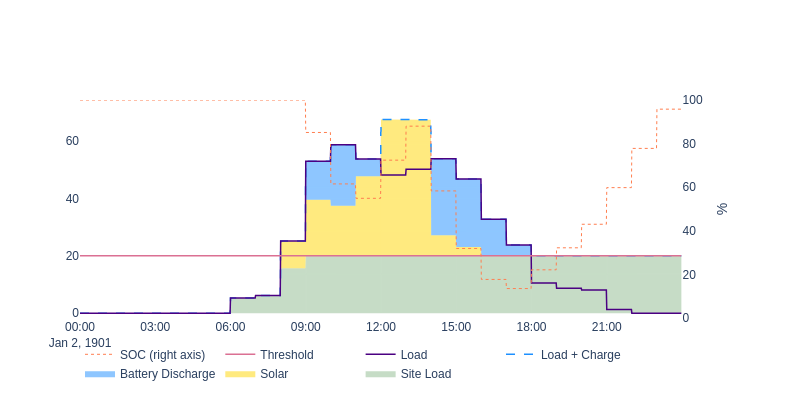
\includegraphics{/home/mjw/Code/Bifacial-solar-and-peakshaving/Paper/images/tech_shaving.png}
\caption{}
\end{figure}

\begin{quote}
\emph{Figure A: The threshold is 20 kW. The battery begins the day full
at 100 kWh. By 8:00 the load has increased above the threshold to 25 kW,
but solar has also increased to 9 kW, so the site load is still below
the threshold. However at 9:00 the battery must discharge at 13 kW to
reduce to site load to 20 kW. At 12:00 the battery can recharge somewhat
due to an increase in solar and slight decrease in load. Then by 18:00
the load is less than the threshold and the battery can recharge,
increasing the site load up to the threshold.}
\end{quote}

An example of technical peak shaving with a threshold of 20 kW is seen
in Figure A. The actual load climbs well above the threshold, but the
solar energy for that day reduces the site load considerably. Battery
discharge is required in the morning and afternoon to keep the site load
below the threshold, with some opportunistic midday charging. The
battery recharges in the evening and overnight.

\hypertarget{economic}{%
\subsubsection{Economic}\label{economic}}

Rather, economic peak shaving aims to reduce what a consumer pays for
power and possibly also energy. Medium and large electric consumers
often pay a price on energy (€\(/kWh\)) and a price on power
(€\(/kWh_{peak}\)), or demand charge. The energy cost
(€\(/kWh \times E_{consumed}\)) may vary with time of day, day of week,
and season of the year, which is often referred to as time of use or
peak pricing. Where there is a sufficient spread between the peak and
off-peak prices there may be the opportunity to curtail load during high
prices, use controllable loads to shift from a high price period to a
lower one, or to use energy storage to buy energy at the lower price and
reduce load during a higher price period. A peak shaving approach
applied to the energy cost could be effective and maybe even
advantageous. However there are several key differences between an
energy based approach and a power one, where peak shaving is better
suited for the latter.

Instead, the power cost (€\(/kW \times P_{max}\) ) typically applies to
the max power during the billing period, where the peak power is the
maximum non-moving average in a given period (e.g. 12:00-18:00 on
weekdays) calculated on a given interval (e.g. 60 minutes). Similar to
the energy cost, there may be multiple time of use periods and
associated prices, such as peak, mid-peak, and off-peak. And where the
spread price is sufficiently high, the period peak can be reduced with
load curtailment or rescheduling, distributed generation such as solar,
or energy storage.

\begin{figure}
\centering
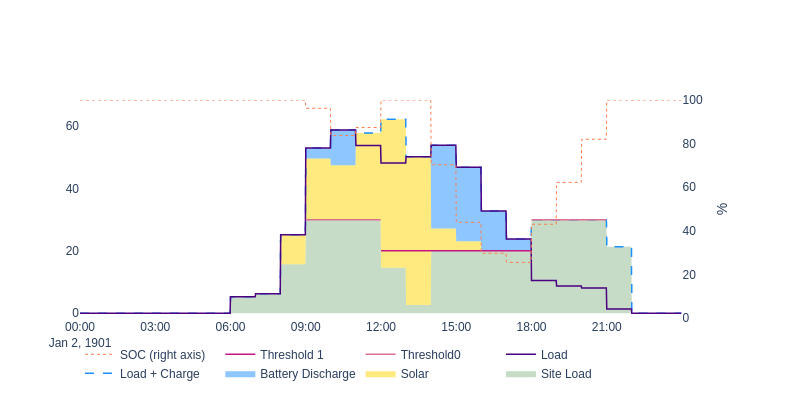
\includegraphics{/home/mjw/Code/Bifacial-solar-and-peakshaving/Paper/images/econ_shaving.png}
\caption{technical peak shaving}
\end{figure}

\begin{quote}
\emph{Figure B: The threshold is comprised of two parts: Threshold0 at
20 kW from 12:00-18:00, and Threshold1 at 40 kW from 9:00-12:00 and
18:00-21:00. The battery begins the day full at 100 kWh. By 9:00 the
load has increased above Threshold0, solar decreases this greatly, and
the battery is discharged to further reduce the site load. However at
9:00 the battery must discharge at 13 kW to reduce to site load to 20
kW. At 11:00 and 12:00 the battery can recharge somewhat due to an
increase in solar and slight decrease in load. Then by 18:00 the load is
significantly less than the threshold and the battery can recharge,
increasing the site load up to the threshold.}
\end{quote}

Solar contributes significantly to the load, but once the peak period
begins the battery must discharge to keep the

\begin{longtable}[]{@{}lll@{}}
\toprule
Feature & Technical Peak Shaving & Economic Peak Shaving\tabularnewline
\midrule
\endhead
Cost of violating the threshold & Prohibitively high & Depends on
tariff\tabularnewline
Averaging interval & \textless\textless{} 1 minute & 15 minutes or 1
hour (typical)\tabularnewline
Valid times of day & All & Limited (e.g. 16:00 to 21:00)\tabularnewline
Peak is reset every.. & Never & Month, year, day
(typical)\tabularnewline
\bottomrule
\end{longtable}

\hypertarget{methodology}{%
\section{Methodology}\label{methodology}}

\begin{figure}
\centering
\includegraphics[width=4.72917in,height=\textheight]{17019648855744.png}
\caption{}
\end{figure}

\begin{quote}
\emph{Figure E: Simplified one-line schematic of the simulated EV
charging station with true measured EV charging power, modelled on-site
solar PV generation, and a modelled stationary battery for economic peak
shaving.}
\end{quote}

The methodology of this study is a set of offline simulations involving
(a) EV charging power measurements, (b) modelled solar PV production
power, and (b) AC-coupled battery dispatch, all behind the retail
electric meter. In each simulation the battery power is chosen such that
the net load (natural load less solar production) is held below a given
threshold, which is optimally chosen by a gradient descent optimizer.
The optimal threshold changes for each TOU period. A single simulation
is defined for one solar configuration and battery capacity and lasts
one calendar month, which is the shortest period for which the cost
function is defined. Simulations are repeated for several months of
data, and many different solar and battery design sizes, allowing for a
retail energy cost comparison among different design scenarios. EV
charging power or solar are never curtailed. The primary decision
variables in each timestep are (a) battery charge or discharge, and (b)
battery power.

\hypertarget{data}{%
\subsection{Data}\label{data}}

\hypertarget{ev-charging-load}{%
\subsubsection{EV Charging Load}\label{ev-charging-load}}

The measured EV charging power ("load") is from the Caltech Adaptive
Charging Network database at the JPL site. Each charging session
provides timeseries active power, averaged over a 10 second interval. In
the cases when complete timeseries data is not available for a session,
the charging profile is estimated and the total charging energy
delivered is the same. The disaggrated session timeseries data is summed
into a single timeseries of total site charging power, which is then
averaged over 15-minute intervals. Timestamp indices refer to the
beginning of the 15-minute interval. The data period is from 2018-5-1
00:00 to 2019-2-28 23:45.

\hypertarget{solar-production}{%
\subsubsection{Solar Production}\label{solar-production}}

The modelled PV production power begins life as GOES satellite solar
irradiance data from the US National Solar Resource Database (NSRDB),
and is specific to the exact time and date rather as opposed to typical
meteorological year data. Prism Solar 350 W bifacial solar module DC
electrical power is estimated using the California Energy Commission
Performance Model, a 6-parameter physical PV cell model. The full AC
array power is estimated given loss assumptions and an inverter
efficiency lookup table in the NREL SAM database for the Enphase IQH 380
W microinverter. All these functions are implemented in SAM v2022.11.21
(Gilman 2015).

Three different solar array orientations are modelled and simulated in
different case studies. Each orientation has the same number and type of
modules: all modules facing South at 20° tilt, all modules facing West
at 90° tilt, and half the modules facing South at 20° tilt and half the
modules facing West at 90° tilt. Tilt is defined as 90° minus the
altitude angle of the normal vector of the primary active face of the
module. No shading is considered. Of the two sides of the bi-facial
module, the primary active face is oriented West since afternoon load is
generally subject to higher prices.

\begin{longtable}[]{@{}lllll@{}}
\toprule
Timeseries Description & Location & Type & Interval / Length &
Source\tabularnewline
\midrule
\endhead
\vtop{\hbox{\strut EV charging power}\hbox{\strut (\(kW_{ac}\))}} & Jet
Propulsion Lab, Pasadena CA, USA & Measured and aggregated from multiple
EV chargers at single site & 10 sec (average downsampled to 15 min) / 10
months & Caltech ACN\tabularnewline
\vtop{\hbox{\strut Solar irradiance }\hbox{\strut (\(W/m^2\))}} & GPS:
34.2013, -118.1721 (2x2 km square) & GOES satellite irradiance & 5
minute / 10 months & NSRDB PSMv3\tabularnewline
PV array production (\(kW_{ac}\)) & GPS: 34.2013, -118.1721 (2x2 km
square) & Modelled from satellite irradiance, 368 Prism Solar 350 W
bifacial modules, 368 Enphase IQH 380 W microinverters & 15 minute / 10
months & SAM (Gilman 2015)\tabularnewline
\bottomrule
\end{longtable}

\begin{quote}
\emph{Table C: Timeseries Data Summary. EV charging power is measured
every 10 seconds for 10 months at the Jet Propulsion Laboratory, CA,
USA. Solar irradiance from the GOES satellite is acquired for the same
location. Solar PV array production is modelled from the satellite
irradiance using a 6 parameter PV cell model and inverter efficiency
lookup table.}
\end{quote}

\hypertarget{battery}{%
\subsection{Battery}\label{battery}}

A stationary, storage battery system is simulated as the primary
decision variable in the peak shaving algorithm. In each timestep the
battery is chosen to charge or discharge within its technical limits.
Because the control action is to hold the power exchange with the grid
to below a certain threshold, batteries with a larger power capacity or
energy capacity will necessarily achieve a lower threshold if the entire
battery capacity is used. For a given energy capacity (\(kWh\)) those
limits are a charge or discharge rate no more than 1C and SOC between 0
and 100\% of rate. Charge and discharge efficiency is assumed constant
and no self discharge or thermal limiting are considered.

There are many strategies for optimal battery sizing, but the emphasis
in this work is instead on understanding the dynamics between load,
shape of the solar curve, and peak shaving algorithm for a given battery
size. Therefore a sensitivity analysis is performed on the battery
energy capacity, but no one battery size is declared economically
optimal.

\begin{longtable}[]{@{}l@{}}
\toprule
Battery Sizes (kWh)\tabularnewline
\midrule
\endhead
25, 50, 75, 100, 125, 150, 200, 400, 600\tabularnewline
\bottomrule
\end{longtable}

\begin{quote}
\emph{Table A: Vector of battery sizes chosen for peak shaving
simulations. These were identified as interesting values
experimentally.}
\end{quote}

Each simulation assumed charge and discharge rate are limited to 1C,
usable SOC is assumed 100\%, and self discharge, parasitic losses, and
thermal limiting are not considered.

\hypertarget{electric-tariff}{%
\subsection{Electric Tariff}\label{electric-tariff}}

A typical California electric tariff is applied at the point of the
retail electric meter, with several different TOU periods and prices.
For the chosen tariff each TOU period may have an energy price
(\(\$/kWh\)), a power price (\(\$/kW\)), or both. The prices may also
change between seasons, and have long term trends like any retail
electric prices. Here a price on power ("demand charge") is understood
as a \(\$/kW\) price applied to the monthly maximum power observed at
the meter, calculated as the 15-minute average of real power.

\begin{longtable}[]{@{}lllll@{}}
\toprule
Name & TOU Period & Summer (Jun 1 - Sept 30) {[}\${]} & Winter (Oct 1 -
Feb 28) {[}\${]} & Spring (Mar 1 - May 30) {[}\${]}\tabularnewline
\midrule
\endhead
All hours & 0:00-0:00 & 26.07 / kW & 26.07 / kW & 26.07 /
kW\tabularnewline
Super off-peak & 9:00-14:00 & -\/- & -\/- & 0.079 / kWh\tabularnewline
Off-peak spring & \vtop{\hbox{\strut 0:00-9:00,
14:00-16:00,}\hbox{\strut 21:00-0:00}} & -\/- & -\/- & 0.132 /
kWh\tabularnewline
Off-peak winter & 0:00-16:00, 21:00-0:00 & -\/- & 0.132 / kWh &
-\/-\tabularnewline
Off-peak summer & 0:00-14:00, 23:00-0:00 & 0.132 / kWh & -\/- &
-\/-\tabularnewline
Partial-peak & 14:00-16:00, 21:00-23:00 & \vtop{\hbox{\strut 6.81 /
kW,}\hbox{\strut 0.159 / kWh}} & -\/- & -\/-\tabularnewline
Peak & 16:00-21:00 & \vtop{\hbox{\strut 32.90 / kW,}\hbox{\strut 0.196 /
kWh}} & \vtop{\hbox{\strut 2.22 / kW,}\hbox{\strut 0.172 / kWh}} &
\vtop{\hbox{\strut 2.22 / kW}\hbox{\strut ,0.172 / kWh}}\tabularnewline
\bottomrule
\end{longtable}

\begin{quote}
\emph{Table B: Retail Electric Tariff. An applicable electric tariff
schedule with seven different TOU periods for energy and power prices,
varying by hours of the day and season of the year. From California
PG\&E.}
\end{quote}

The total retail electric cost \(C\) for each month is then the sum of
the energy cost and power cost for the month, where the energy and power
costs are calculated separately for each TOU period. The energy cost is
the energy delivered to the site multiplied by the energy price for that
TOU period. The power cost is the maximum 15-minute average power for
the month multiplied by the power price for that TOU period.

\begin{equation}
\begin{split}
NL(t) &= L(t) - S(t) \\
NL_{p}(t) &= NL(t),\ \forall \ NL(t)>0 \\
B(t) &= B_d(t) - B_c(t) \\
C_m &= \Sigma_k^K [ p_{p,k,m} max(NL_{p,k,m}-B) + p_{e,k,m} \Sigma (NL_{p,k,m}-B) ] \\
\\
& \text{where:} \\
&L \text{ is EV charging load}\ (kW) \\
&S \text{ is solar production}\ (kW)\\
&NL \text{ is net load}\ (kW) \\
&B_c \text{ is battery charging power (non-negative)}\ (kW) \\
&B_d \text{ is battery discharging power (non-negative)}\ (kW) \\
&C_m \text{ is total retail electric cost for month}\ m\ (\$) \\
&p_{p,k,m} \text{ is power price for TOU period}\ k\ \text{and month}\ m\  (\$/kW) \\
&p_{e,k,m} \text{ is energy price for TOU period}\ k\ \text{and month}\ m\ (\$/kWh) \\
&K \text{ is number of TOU periods}
\end{split}
\end{equation}

\hypertarget{peak-shaving-algorithm}{%
\subsection{Peak Shaving Algorithm}\label{peak-shaving-algorithm}}

An optimal peak shaving strategy is used to minimized the total retail
electric cost to the EV charging station. The strategy is operational
only, and assumes the solar production timeseries and battery capacity
are fixed. The state variable controlled by the algorithm is battery
charge or discharge power. However the algorithm reframes the problem as
one of choosing a power threshold \(T\ (kW)\) applied to the point of
injection to the grid, the electric meter. The battery is then
dispatched, within its technical limits, to hold the net load (natural
load less solar production) below the threshold. When the algorithm is
successful the different thresholds for each TOU period are met for an
entire month. If the battery reaches a technical limit and net load
exceeds a threshold, the simulation is not necessarily invalid but is
not likely to minimize the retail electric cost to the site for that
combination of solar and battery size. The peak shaving logic is
described in Figure D.

\begin{figure}
\centering
\includegraphics[width=6.59375in,height=\textheight]{17019648855825.png}
\caption{}
\end{figure}

\begin{quote}
\emph{Figure D: Peak shaving dispatch. Net load is the timeseries of
load less solar. There is one threshold value for one for each TOU
period with a non-zero power price. For each timestep of the simulation
the net load is compared to the threshold of that TOU period, and the
battery is discharged if the net load is greater than the threshold and
charged if the net load is less than the threshold. If the two are equal
the battery does nothing. For timesteps with no price on power the the
battery does nothing.}
\end{quote}

The peak shaving algorithm describes stepping through time and
dispatching the battery according to power thresholds, but not how the
thresholds are chosen.

\hypertarget{threshold-optimizer}{%
\subsection{Threshold Optimizer}\label{threshold-optimizer}}

The optimal demand thresholds (one per TOU period) are determined by a
custom gradient descent optimizer. The objective function \(C\)
minimizes the retail energy cost of one month, which is the billing
interval of this retail electric tariff. In practice the optimal
thresholds are different for each month. The threshold for each TOU
period \(T_k\) is not enforced to be non-negative, but in practice is
always is because the cost function \(C_m()\) cannot evaluate to a
negative value.

\begin{equation}
\begin{split}
min[C_m(B_c,B_d)] & = min[C_m(T_1,T_2,..T_K)] \\
& s.t. \\
B_c(t) & \le B_{c,max} \\
B_d(t) & \le B_{d,max} \\
SOC_{min} & \le SOC(t) \le SOC_{max} \\
\\
& \text{where:} \\
B_c & \text{ is battery charge power timeseries}\ (kW) \\
B_d & \text{ is battery discharge power timeseries}\ (kW) \\
T_k & \text{ is threshold for}\ k\text{-th TOU period of}\ K\ \text{total periods} \\
SOC & \text{ is battery state of charge timeseries}\ (\frac{kWh}{kWh}) \\
\end{split}
\end{equation}

Beginning from an initial guess the Newton-Raphson gradient descent
optimizer calculates the batch gradient and updates parameters based on
a learning rate of 0.01. This continues until the stopping condition is
met, minimum cost for a patience of 50 iterations. The Newton-Raphson
gradient descent based optimization method is preferred over linear
programming because it will minimize over a variety of cost functions
without needing to reformulate the linear program.

\hypertarget{simulations}{%
\subsection{Simulations}\label{simulations}}

Simulations are run one month at a time for a given solar array
orientation and battery capacity, according to the flowchart in Figure
C. The computational environment is Python 3.8 in Windows 10 64-bit, on
an Intel i9 CPU with 64 GB of RAM.

\begin{figure}
\centering
\includegraphics[width=3.64583in,height=\textheight]{17019648855896.png}
\caption{}
\end{figure}

\begin{quote}
Figure C: Simulation Flowchart. Given a solar orientation and chosen
battery capacity, the net load timeseries is calculated from EV charging
load and solar production. The threshold optimizer produces one
threshold value (kW) for each TOU period with non-zero power prices.
This returns both optimal thresholds and a minimum cost. Lastly a 1
month simulation of the battery charging and discharging is performed to
ensure no violations of the battery technical limits, and to produce the
battery power timeseries for evaluation.
\end{quote}

\hypertarget{case-studies}{%
\section{Case Studies}\label{case-studies}}

Three case studies are evaluated, each relating to the orientation of
the solar array but not changing the overall \(kWp\) capacity. All case
studies use the Prism 350 W bifacial solar PV modules and the Enphase
IQH 380 W microinverters.

The first and baseline case is a South-facing array of 368 modules,
tilted at 20˚. This is intended to be a typical rooftop solar plant,
especially in northern latitudes where lower sun angles and winter snow
make the research question of vertical bifacial modules even more
relevant. The daily clearsky solar power curve is the familiar rounded
triangle centered at solar noon. The array is sized such that the total
energy produced is equal to the total energy consumption of the EV
charging station. This "net zero" sizing is not necessarily economically
optimal, but rather it is a reasonable or typical size solar plant for
the load.

The second case instead orients the active high-power face of the
bifacial module West and tilts the module vertically at 90˚. This is an
extreme case, especially at this large number of modules, but should be
investigated since it represents the maximum amount that the daily
clearsky power curve can be pushed toward the morning and evening from
solar noon, making a two-peaked M-shape curve.

The third case only orients half the modules West and 90°, which is a
linear combination of the first two cases and physically represents a
more realistic physical design. The motivation for including this case
in the investigation is that while the time of solar production is
important for peak shaving, too much production in a small later
afternoon window may not be well timed with the late afternoon peak and
more energy overall would have been sufficient.

\begin{longtable}[]{@{}lllll@{}}
\toprule
Case & Orientation & Tilt & \vtop{\hbox{\strut Total Energy
}\hbox{\strut {[}\(MWh\){]}}} & \vtop{\hbox{\strut Solar
Yield}\hbox{\strut  {[}\(\frac{kWh}{kW_p}\){]}}}\tabularnewline
\midrule
\endhead
1 (baseline) & South (368 modules) & 20° & 151.7 & 1180.8\tabularnewline
2 & West (368 modules) & 90° & 131.0 & 1019.3\tabularnewline
3 & \vtop{\hbox{\strut South (184 modules)}\hbox{\strut West (184
modules)}} & \vtop{\hbox{\strut 20°}\hbox{\strut 90°}} & 141.1 &
1098.2\tabularnewline
\bottomrule
\end{longtable}

\begin{quote}
\emph{Table D: Case Studies. All modules are the Prism 350 W bifacial.
The baseline Case 1 is a South-facing array tilted to 20°. In Case 2 the
primary high power surface faces West and the modules are tilted to 90°.
In Case 3 half the array modules face West and are tilted at 90˚, and
half the modules face South and are tilted at 20˚.}
\end{quote}

\hypertarget{results}{%
\section{Results}\label{results}}

The peak shaving methodology produces an optimally low retail electric
cost for each of the 10 months of data, which are summed up for total
electric cost in Figure A versus the battery capacity sensitivity
analysis. The costs monotonically decrease with battery capacity as
expected because every marginal unit of added battery energy capacity
allows the algorithm to hold a power threshold for longer, and since
each battery is rated for 1C at charging and discharging, the battery
will also have more power capacity to achieve lower thresholds relative
to the same size peak. The West 90° array never achieves a lower total
cost than the baseline South 20°. The combination South 20° / West 90°
array does for all battery sizes below 400 kWh, with a maximum reduction
of \$1120 (3.05\%) relative to the South 20° at a very small battery
size of 50 kWh. The largest percentage improvement of 3.54\% (\$890)
occurs for the 125 kWh battery. The absolute cost reduction is likely
more important than the relative reduction since it would be treated
directly as revenue in a cash flow analysis to determine the economic
performance of a given battery.

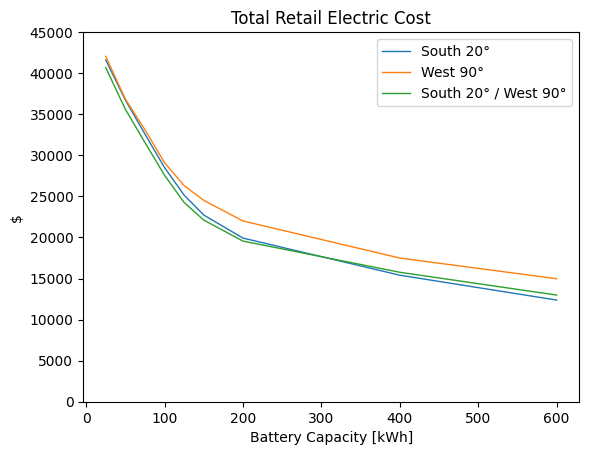
\includegraphics{/home/mjw/Code/Bifacial-solar-and-peakshaving/Paper/images/total retail electric cost.png}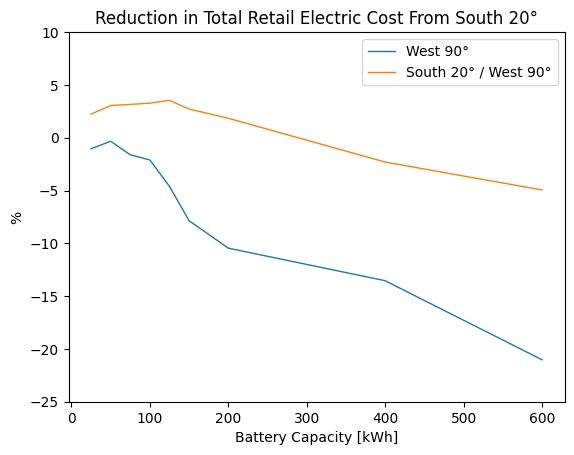
\includegraphics{/home/mjw/Code/Bifacial-solar-and-peakshaving/Paper/images/reduction in total retail electric cost.png}

\begin{quote}
\textbf{Figure A: Total Retail Electric Cost and Percentage Reduction.}
Left: The West 90° array does not reduce the total cost compared to the
baseline South 20°array, but the combination South 20°/ West 90° array
with 50 kWh battery does reduce the cost \$1120 (3.05\%) over the 10
month data period. Right: The largest percentage decrease in total cost
is 3.54\% (\$890) for the 125 kWh battery.
\end{quote}

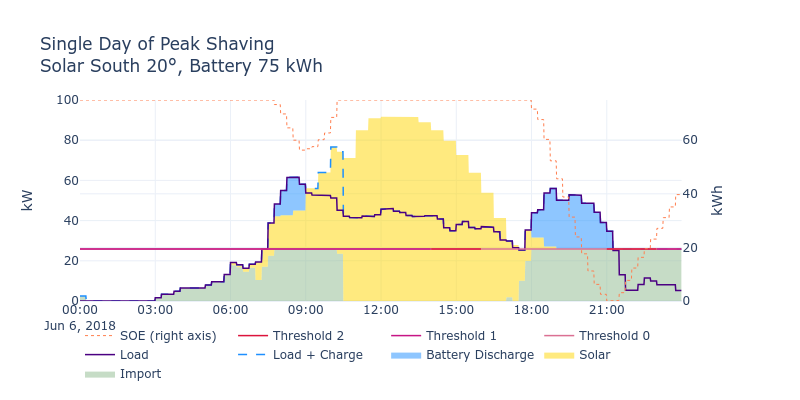
\includegraphics{/home/mjw/Code/Bifacial-solar-and-peakshaving/Paper/images/single day of peak shaving 1.png}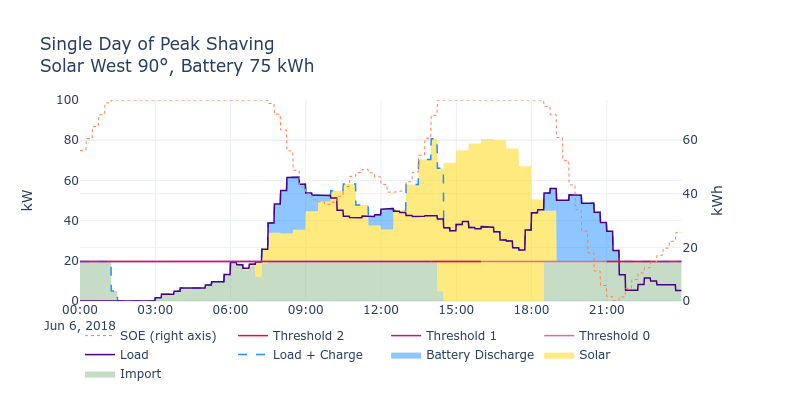
\includegraphics{/home/mjw/Code/Bifacial-solar-and-peakshaving/Paper/images/single day of peak shaving 2.png}

\begin{quote}
\textbf{Figure F: Single Day of Peak Shaving.} Left: The South 20° solar
array overproduces during the middle hours of the day but falls to 28 kW
while the evening peak
\end{quote}

\begin{longtable}[]{@{}llllllll@{}}
\toprule
Battery Capacity (kWh) & \vtop{\hbox{\strut South 20°
}\hbox{\strut (Baseline)}} & West 90° & \vtop{\hbox{\strut 50\% South
20°}\hbox{\strut 50\% West 90°}} & \vtop{\hbox{\strut West
90°}\hbox{\strut Reduction}} & \vtop{\hbox{\strut 50\% South
20°}\hbox{\strut 50\% West 90° }\hbox{\strut Reduction}} &
\vtop{\hbox{\strut West 90°}\hbox{\strut Reduction}\hbox{\strut \%}} &
\vtop{\hbox{\strut 50\% South 20°}\hbox{\strut 50\% West 90°
}\hbox{\strut Reduction \%}}\tabularnewline
\midrule
\endhead
25 & 29588.0 & 29221.0 & 29133.0 & 367.0 & 455.0 & 1.24 &
1.53\tabularnewline
50 & 23747.0 & 22972.0 & 22876.0 & 775.0 & 871.0 & 3.26 &
3.66\tabularnewline
75 & 19797.0 & 18721.0 & 19058.0 & 1076.0 & 739.0 & 5.43 &
3.73\tabularnewline
100 & 16230.0 & 15495.0 & 15279.0 & 735.0 & 951.0 & 4.52 &
5.85\tabularnewline
125 & 13388.0 & 12682.0 & 12454.0 & 706.0 & 934.0 & 5.27 &
6.97\tabularnewline
150 & 11155.0 & 11112.0 & 10519.0 & 43.0 & 636.0 & 0.38 &
5.70\tabularnewline
200 & 8445.0 & 8715.0 & 8017.0 & -270.0 & 428.0 & -3.19 &
5.06\tabularnewline
400 & 4850.0 & 5372.0 & 5024.0 & -522.0 & -174.0 & -10.76 &
-3.58\tabularnewline
600 & 3694.0 & 4180.0 & 3807.0 & -486.0 & -113.0 & -13.15 &
-3.05\tabularnewline
\bottomrule
\end{longtable}

Table C: Battery size sensitivity analysis for each of the two solar
configuration cases, standard rate tariff

\begin{longtable}[]{@{}lll@{}}
\toprule
Solar Capacity (\% of net zero) & Best s20-\textgreater w90 Reduction
{[}\$,\%{]} (Batt {[}kWh{]}) & Best s20-\textgreater s20w90 Reudction
{[}\$,\%{]} (Batt {[}kWh{]})\tabularnewline
\midrule
\endhead
50\% & 183, 0.6\% (25) & 360, 1.1\% (25)\tabularnewline
100\% & 1076, 5.4\% (75) & 951, 5.9\% (100)\tabularnewline
125\% & 1158, 7.0\% (75) & 1091, 5.6\% (75)\tabularnewline
150\% & 1527, 7.9\% (75) & 1281, 8.4\% (100)\tabularnewline
175\% & 1621, 13.5\% (125) & 1668, 13.9\% (125)\tabularnewline
200\% & 1618, 13.9\% (125) & 1656, 14.2\% (125)\tabularnewline
\bottomrule
\end{longtable}

Table D: Solar capacity sensitivity analysis fo

\hypertarget{conclusion}{%
\section{Conclusion}\label{conclusion}}

\hypertarget{bibliography}{%
\section{Bibliography}\label{bibliography}}

\end{document}
